%%%%%%%%%%%%%%%%%%%%%%%%%%%%%%%%%%%%%%%%%
% Jacobs Landscape Poster
% LaTeX Template
% Version 1.1 (14/06/14)
%
% Created by:
% Computational Physics and Biophysics Group, Jacobs University
% https://teamwork.jacobs-university.de:8443/confluence/display/CoPandBiG/LaTeX+Poster
% 
% Further modified by:
% Nathaniel Johnston (nathaniel@njohnston.ca)
%
% This template has been downloaded from:
% http://www.LaTeXTemplates.com
%
% License:
% CC BY-NC-SA 3.0 (http://creativecommons.org/licenses/by-nc-sa/3.0/)
%
%%%%%%%%%%%%%%%%%%%%%%%%%%%%%%%%%%%%%%%%%

%----------------------------------------------------------------------------------------
%	PACKAGES AND OTHER DOCUMENT CONFIGURATIONS
%----------------------------------------------------------------------------------------

\documentclass[final]{beamer}

\usepackage[scale=1.24]{beamerposter} % Use the beamerposter package for laying out the poster

\usetheme{confposter} % Use the confposter theme supplied with this template

% \setbeamercolor{block title}{fg=ngreen,bg=white} % Colors of the block titles
% \setbeamercolor{block body}{fg=black,bg=white} % Colors of the body of blocks
% \setbeamercolor{block alerted title}{fg=white,bg=dblue!70} % Colors of the highlighted block titles
% \setbeamercolor{block alerted body}{fg=black,bg=dblue!10} % Colors of the body of highlighted blocks
% Many more colors are available for use in beamerthemeconfposter.sty

%-----------------------------------------------------------
% Define the column widths and overall poster size
% To set effective sepwid, onecolwid and twocolwid values, first choose how many columns you want and how much separation you want between columns
% In this template, the separation width chosen is 0.024 of the paper width and a 4-column layout
% onecolwid should therefore be (1-(# of columns+1)*sepwid)/# of columns e.g. (1-(4+1)*0.024)/4 = 0.22
% Set twocolwid to be (2*onecolwid)+sepwid = 0.464
% Set threecolwid to be (3*onecolwid)+2*sepwid = 0.708

\newlength{\sepwid}
\newlength{\onecolwid}
\newlength{\twocolwid}
\newlength{\threecolwid}
\setlength{\paperwidth}{48in} % A0 width: 46.8in
\setlength{\paperheight}{36in} % A0 height: 33.1in
\setlength{\sepwid}{0.024\paperwidth} % Separation width (white space) between columns
\setlength{\onecolwid}{0.22\paperwidth} % Width of one column
\setlength{\twocolwid}{0.464\paperwidth} % Width of two columns
\setlength{\threecolwid}{0.708\paperwidth} % Width of three columns
\setlength{\topmargin}{-0.5in} % Reduce the top margin size
%-----------------------------------------------------------

\usepackage{graphicx}  % Required for including images

\usepackage{booktabs} % Top and bottom rules for tables

%----------------------------------------------------------------------------------------
%	TITLE SECTION 
%----------------------------------------------------------------------------------------

\title{Hardware Acceleration of Networking Encryption Algorithm AES in GCM } % Poster title

\author{Yu Cao\inst{1}} % Author(s)
\institute{$^1$New York University} % Institution(s)

% \institute{$^1$New York University~~$^2$New York University Abu Dhabi~~$^3$New York University Shanghai} % Institution(s)

%----------------------------------------------------------------------------------------

\begin{document}

\addtobeamertemplate{block end}{}{\vspace*{2ex}} % White space under blocks
\addtobeamertemplate{block alerted end}{}{\vspace*{2ex}} % White space under highlighted (alert) blocks

\setlength{\belowcaptionskip}{2ex} % White space under figures
\setlength\belowdisplayshortskip{2ex} % White space under equations

\begin{frame}[t] % The whole poster is enclosed in one beamer frame

\begin{columns}[t] % The whole poster consists of three major columns, the second of which is split into two columns twice - the [t] option aligns each column's content to the top

\begin{column}{\sepwid}\end{column} % Empty spacer column

\begin{column}{\onecolwid} % The first column

%----------------------------------------------------------------------------------------
%	OBJECTIVES
%----------------------------------------------------------------------------------------

\begin{alertblock}{Motivations}

Datacenters are massively deployed with fast and large throughput networks. Packet payload encryption costs too many CPUs. 
\begin{itemize}
\item Fifteen cores to achieve 40 Gb/s full duplex AES-GCM encryption.
\item A core in its life can earn estimiated \textbf{\emph{4,500\$}}.
\item AES-GCM is massively parallel and its primitives are hardware friendly.
% \item Euismod non erat. Nam ultricies pellentesque nunc, ultrices volutpat nisl ultrices a.
\end{itemize}

\end{alertblock}

%----------------------------------------------------------------------------------------
%	INTRODUCTION
%----------------------------------------------------------------------------------------

\begin{block}{Advanced Encryption Standard}

The AES\cite{daemen2013design} encryption algorithm was first developed in the early 2000. It is now widely used as it is easy to implement and has a robust security. AES is an iterative  encryption method that is symmetric, which means same key can encrypt and decrypt the text.
It is easy to implement both on the software and the hardware due to its intrinsic parallel operational structures shown in fig. \ref{fig:aes}. 

\end{block}

%------------------------------------------------

\begin{figure}
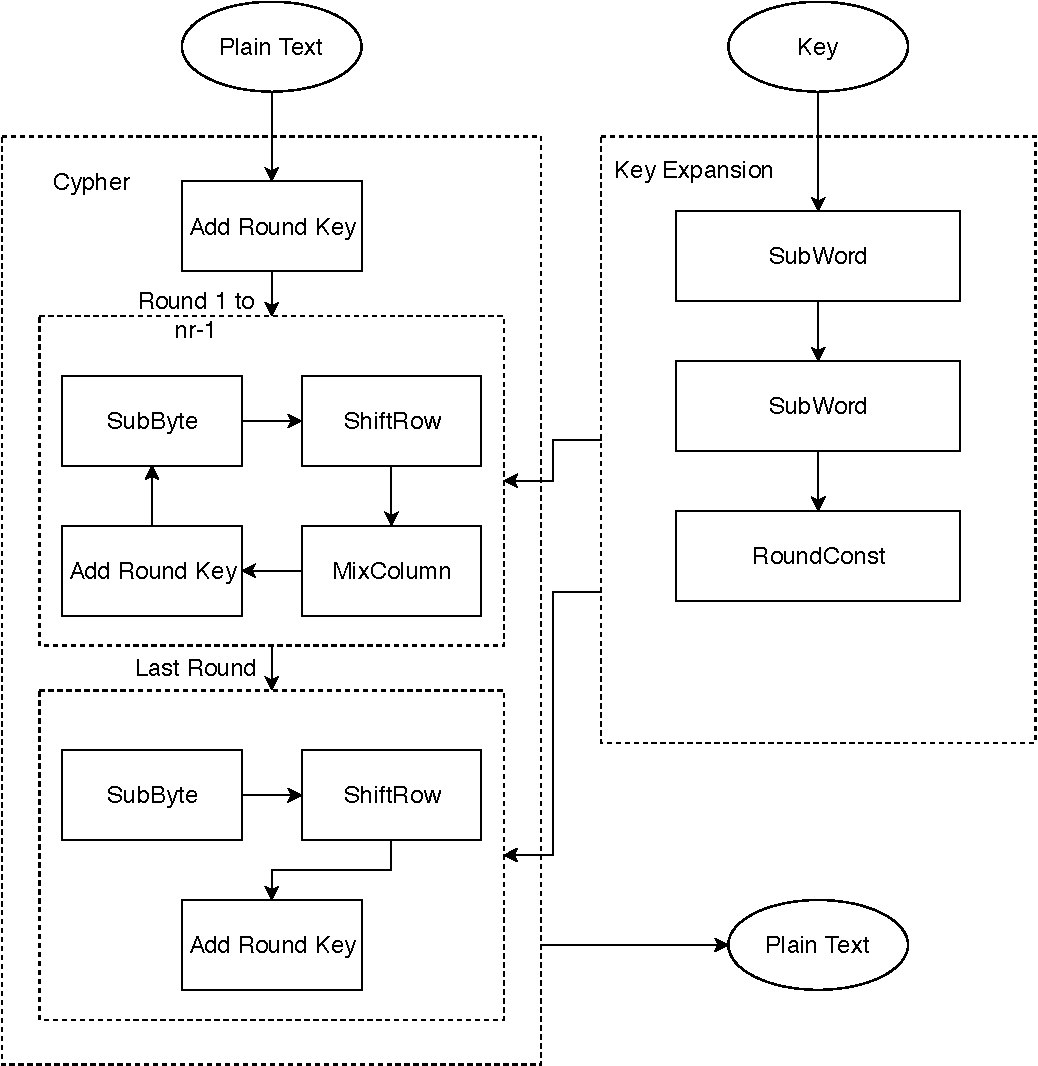
\includegraphics[width=1\linewidth]{poster/AES_paper.pdf}
\caption{AES}
\label{fig:aes}
\end{figure}

%----------------------------------------------------------------------------------------

\end{column} % End of the first column

\begin{column}{\sepwid}\end{column} % Empty spacer column

\begin{column}{\twocolwid} % Begin a column which is two columns wide (column 2)

\begin{columns}[t,totalwidth=\twocolwid] % Split up the two columns wide column

\begin{column}{\onecolwid}\vspace{-.6in} % The first column within column 2 (column 2.1)

%----------------------------------------------------------------------------------------
%	MATERIALS
%----------------------------------------------------------------------------------------

\begin{block}{Galois/Counter Mode}

\begin{figure}
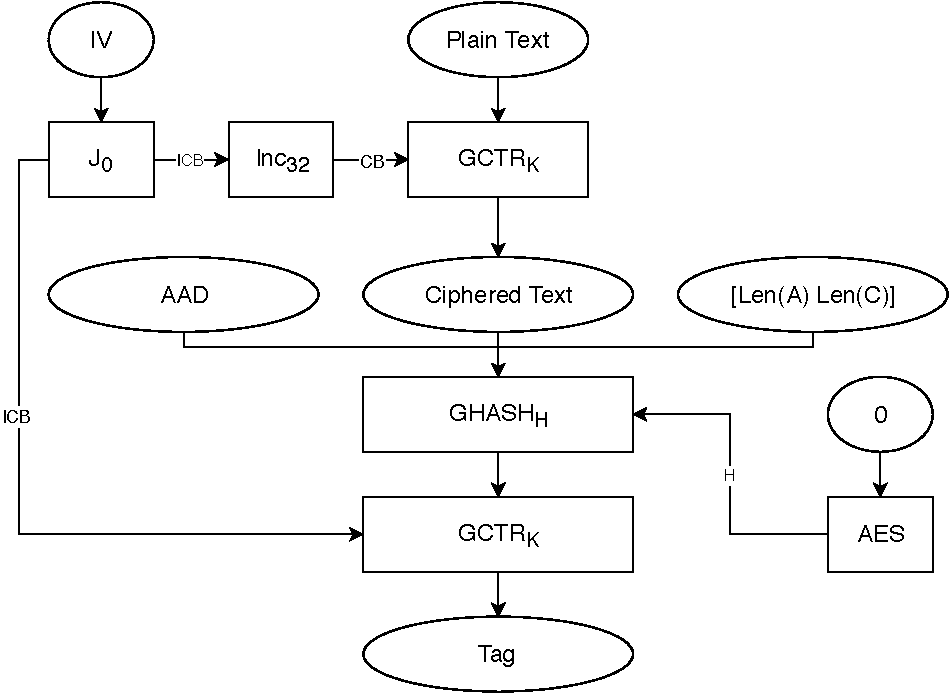
\includegraphics[width=1\linewidth]{poster/GCM.pdf}
\caption{GCM}
\label{fig:gcm}
\end{figure}
GCM works in a rotated counter scheme. It generates cyphered text as well as a Tag/MAC (Message Authentication Code) on data which is not encrypted. The round counter machanism and the additional authentication code add robustness to the encryption system while only bring reasonable overhead.
Fig. \ref{fig:modes} shows that we use AES in GCM code because of the round encryption scheme.

The AES-GCM encryption is implemented as a bump-in-the-wire on the back-
bone of the reference switch design implementation on the NetFPGA platform shown in \ref{impl}.
% The testbed FPGA has four 10 Gbits/s ports, two of which are connected to 2
% NICs in the motherboard to serve as the transmitting and receiving ends.
The slacks vary from \textbf{0.078ns} to \textbf{0.298ns} in \textbf{5.000ns} time window.

\end{block}

%----------------------------------------------------------------------------------------

\end{column} % End of column 2.1

\begin{column}{\onecolwid}\vspace{-.6in} % The second column within column 2 (column 2.2)


%----------------------------------------------------------------------------------------
%	METHODS
%----------------------------------------------------------------------------------------

\begin{block}{Methods}

\begin{figure}

\includegraphics[width=\linewidth]{poster/aes_gcm.png}
\caption{Original, AES and AES-GCM}
\label{fig:modes}
\end{figure}


In the first phase,the AES-GCM is implemented in fully pipeline fashion as shown in fig. \ref{impl}. The implementation has in total 15 clocks of pipeline stages. In the pipeline, this design can process 128-bit data one of a time, meaning 128-bit of input data(either AAD or plaintext) will be processed after 15 clks. 

The crypto module  is inserted before the FPGA switch output the packet. the data is transmitted in AXI Stream with 256-bit data chunks. Since the block cipher encrypts every 128-bit block incrementally and the first 112-bit is the header, the mechanism shown in fig. \ref{fig:paral} is used for 2 AES-GCM module encrypting the data in parallel.


\begin{figure}
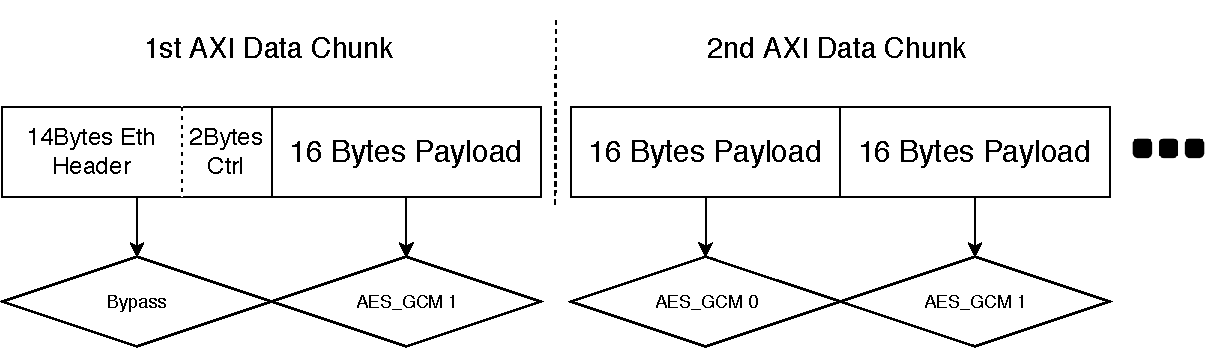
\includegraphics[width=\linewidth]{poster/crypto.pdf}
\caption{Encryption Modules}

\label{fig:paral}
\end{figure}

% A demo is running to  send any message to the other end by encrypted or plaintext modes.

\end{block}

%----------------------------------------------------------------------------------------

\end{column} % End of column 2.2

\end{columns} % End of the split of column 2 - any content after this will now take up 2 columns width


%----------------------------------------------------------------------------------------
\begin{figure}
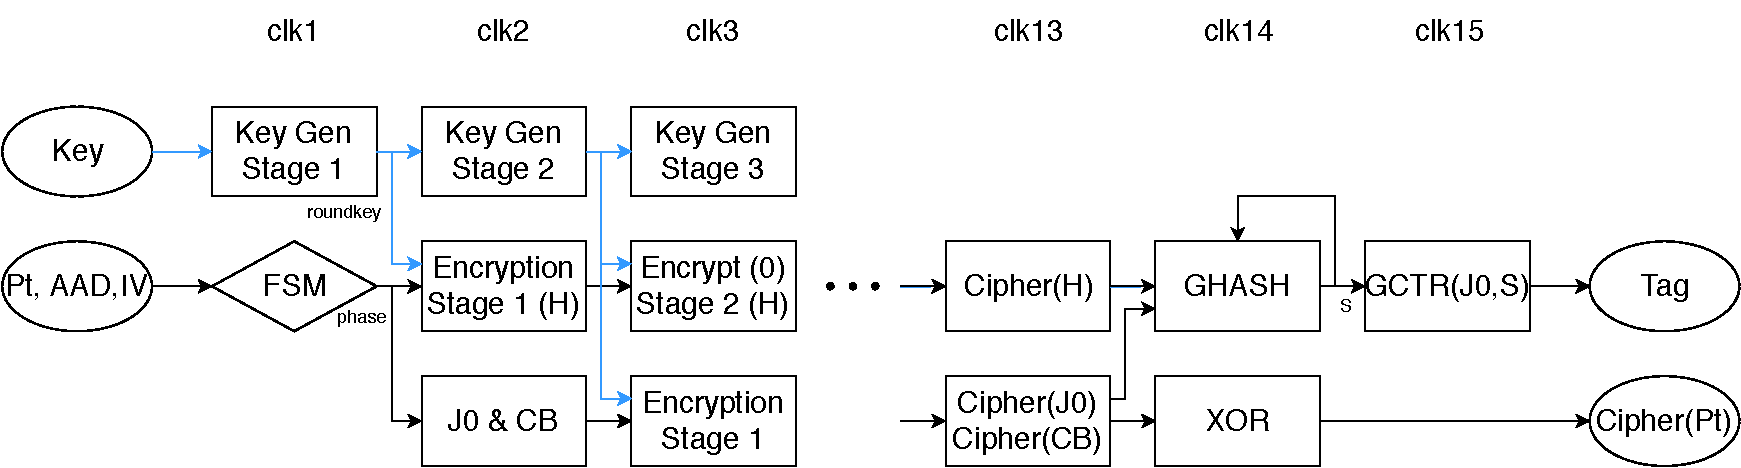
\includegraphics[width=1\linewidth]{poster/aes_gcm_fpga.pdf}
\caption{Implementation of AES-GCM}
\label{impl}
\end{figure}

\end{column} % End of the second column

\begin{column}{\sepwid}\end{column} % Empty spacer column

\begin{column}{\onecolwid} % The third column

%----------------------------------------------------------------------------------------
%	CONCLUSION
%----------------------------------------------------------------------------------------

\begin{block}{Experiments}

Table \ref{comp} makes a rough comparison between our FPGA implementation and CPU implementation according to the statistics from paper \cite{caulfield2016cloud}.

\begin{table}
\vspace{2ex}
\begin{tabular}{ccc}
\toprule
 & \textbf{CPU} & \textbf{FPGA}\\
\midrule
Frequency(MHz) & 4000 & 200\\
Latency(ns) & 4000 & 75 \\
Power(W)  & 50 & 7.5 \\
\bottomrule
\end{tabular}
\caption{Comparison between CPU and FPGA}
\label{comp}
\end{table}

Table \ref{util} shows the implementation utilization results.

\begin{table}
\vspace{2ex}
\begin{tabular}{cccc}
\toprule
 & \textbf{Used} & \textbf{Avalaible} & \textbf{Percentage} \\
\midrule
LUTs & 23088 & 108300 & 21.32\%\\
Registers  & 75512 & 866400 & 8.72\% \\
BRAM(MB) & 272.5 & 1470 & 18.54\% \\
\bottomrule
\end{tabular}
\caption{Utilization}
\label{util}
\end{table}

\end{block}

%----------------------------------------------------------------------------------------
%	ADDITIONAL INFORMATION
%----------------------------------------------------------------------------------------

\begin{block}{Future Work}

\begin{itemize}
\item Do tag generation in 2 AES-GCM pipelines.
\item Further optimize the pipeline.
% \item Duis porta consequat lorem
\end{itemize}

\end{block}

%----------------------------------------------------------------------------------------
%	REFERENCES
%----------------------------------------------------------------------------------------

\begin{block}{References}

% \nocite{*} % Insert publications even if they are not cited in the poster
\small{\bibliographystyle{unsrt}
\bibliography{sample}\vspace{0.75in}}
\begin{center}
\begin{tabular}{ccc}

\includegraphics[width=\linewidth]{nyu-logo} % change to nyu-logo and nyush-logo accordingly
\end{tabular}
\end{center}
\end{block}

%----------------------------------------------------------------------------------------
%	ACKNOWLEDGEMENTS
%----------------------------------------------------------------------------------------

% % \setbeamercolor{block title}{fg=red,bg=white} % Change the block title color
% \begin{center}
% \begin{tabular}{ccc}
% 
\includegraphics[width=\linewidth]{nyu-logo} % change to nyu-logo and nyush-logo accordingly
% \end{tabular}
% \end{center}

%----------------------------------------------------------------------------------------

\end{column} % End of the third column

\end{columns} % End of all the columns in the poster

\end{frame} % End of the enclosing frame

\end{document}
